\documentclass[tikz,border=2pt]{standalone}
\usepackage{amsmath,amssymb}
\usepackage{tikz}
\usetikzlibrary{arrows.meta}

\begin{document}
% For symmetric A = [[2,1],[1,2]] (eigenvalues 3 and 1, both positive) the set x^T A x = 1 is
% an ellipse whose axes are the eigenvectors, with half-lengths 1/sqrt(lambda).
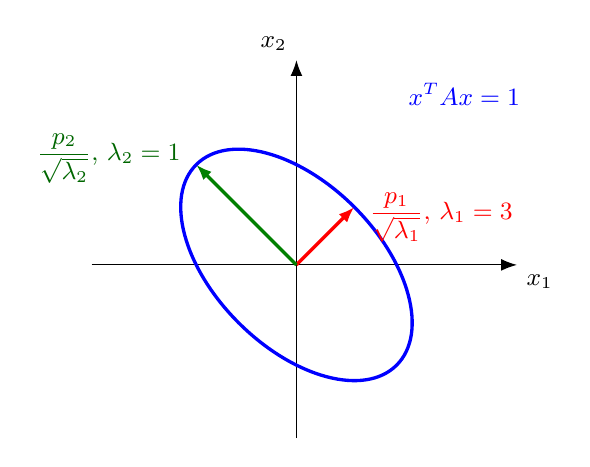
\begin{tikzpicture}[every node/.style={font=\small}, >={Latex[length=2mm]}]
	\draw[->] (-2.6,0) -- (2.8,0) node[below right] {$x_1$};
	\draw[->] (0,-2.2) -- (0,2.6) node[above left] {$x_2$};
	\begin{scope}[rotate=45, scale=1.8]
		\draw[blue, very thick] (0,0) ellipse ({1/sqrt(3)} and 1);
		\draw[->, red, very thick] (0,0) -- ({1/sqrt(3)},0);
		\draw[->, green!50!black, very thick] (0,0) -- (0,1);
	\end{scope}
	\node[red, anchor=west] at (0.8,0.6) {$\dfrac{p_1}{\sqrt{\lambda_1}}$, $\lambda_1=3$};
	\node[green!40!black, anchor=east] at (-1.35,1.35) {$\dfrac{p_2}{\sqrt{\lambda_2}}$, $\lambda_2=1$};
	\node[blue, anchor=south west] at (1.3,1.9) {$x^{T}Ax=1$};
\end{tikzpicture}
\end{document}
